% major update 8/4/11
% typo fixes 12/5/11
% --------------------------------------------------------------------------
%\documentclass[onecolumn,11pt]{ieeetran}
\documentclass[]{siamltex}
\usepackage{graphics,amssymb,amsmath,amsfonts,epsfig} %stfloats
%\usepackage{algorithm}
%\usepackage{algorithmic}
\usepackage{hyperref}
\usepackage{verbatim}
%\usepackage[named]{algo}

% Example definitions
% -------------------
\def\x{{\mathbf x}}
\def\L{{\cal L}}
\def\half{\frac{1}{2}}
\def\alphamax{\alpha_{\mbox{\tiny max}}}
\def\alphamin{\alpha_{\mbox{\tiny min}}}


% more useful abbreviations
% -------------------------
\newcommand{\R}{\mathbb{R}}
\newcommand{\C}{\mathbb{C}}
\newcommand{\btheta}{\mbox{\boldmath $\theta$}}
\newcommand{\bgamma}{\mbox{\boldmath $\gamma$}}
\newcommand{\bbeta}{\mbox{\boldmath  $\beta$}}
\newcommand{\balpha}{\mbox{\boldmath $\alpha$}}
\newcommand{\bDelta}{\mbox{\boldmath $\Delta$}}
\newcommand{\bdelta}{\mbox{\boldmath $\delta$}}
\newcommand{\bPsi}{\mbox{\boldmath   $\Psi$}}
\newcommand{\bphi}{\mbox{\boldmath   $\phi$}}
\newcommand{\bpi}{\mbox{\boldmath    $\pi$}}
\newcommand{\btau}{\mbox{\boldmath   $\tau$}}
\newcommand{\blambda}{\mbox{\boldmath $\lambda$}}
\newcommand{\bTheta}{\mbox{\boldmath $\Theta$}}
\newcommand{\bone}{\mbox{\boldmath   $1$}}
\newcommand{\Loewner}[0]{\preceq}
\newcommand{\Hessmat}{{\cal H}}
\newcommand{\Bmat}{{\bf B}}
\newcommand{\Amat}{{\bf A}}
\newcommand{\bx}{{\bf x}}
\newcommand{\gradv}{{\bf g}}
\newcommand{\cG}{{\cal G}}
\newcommand{\cS}{{\cal S}}
\newcommand{\cT}{{\cal T}}
\newcommand{\trace}{\mbox{\rm trace}}
\newcommand{\tv}{\tilde{v}}
\newcommand{\gammaC}{\gamma_C}

\def\noprint#1{}
\def\swcomment#1{{\em [SW: #1]}}
\def\dmcomment#1{{\em [DM: #1]}}
\def\swresolved#1{}
\def\dmresolved#1{}
\def\sparsa{SpaRSA\ }
\def\bi{\begin{itemize}}
\def\ei{\end{itemize}}
\def\beq{\begin{equation}}
\def\eeq{\end{equation}}
\def\eqnok#1{(\ref{#1})}

% theorem environments
% \newtheorem{theorem}{Theorem}
% \newtheorem{lemma}[theorem]{Lemma}
% \newtheorem{corollary}[theorem]{Corollary}

% baselinestretch definition is important!!
% \renewcommand{\baselinestretch}{1.565}

% \ninept

% Title.
% ------
\title{EECS 451 Fall 2013 HW 9 \\
 \hspace{1.2cm} Due December 10}
 \date{}

\begin{document}
%\ninept
%
\maketitle

After a genuine attempt to solve the homework problems by yourself, you are free to collaborate with your fellow students to find solutions to the homework problems. Regardless of whether you collaborate with other 451 students, you are required to write your own solutions to hand in. Copying homework solutions from another student or from existing solutions will be considered a violation of the honor code. Finally, if you choose to collaborate, you must include the names of your collaborators on your submitted homework. I haven't figured out yet how to track this, but I do look at it every once in awhile to see who's working with whom.

\vspace{2mm} 

Please take advantage of the Piazza discussion forum on CTools and the professor's and GSI's office hours. This is a pretty easy one, though...

\vspace{2mm}
All HWs are worth 50 points. Each problem is worth 10 points.

\vspace{5mm}

\begin{enumerate}

\item Suppose the input-output relation of a system is given as 
\begin{equation}
y[n] = \sum_{k=0}^M b_k x[n-k] + \sum_{k=1}^N a_k y[n-k]\;.\label{diff}
\end{equation} Show that the Z-transform of the impulse response $h[n]$ is equal to $$H(z) = \frac{\sum_{k=0}^M b_k z^{-k}}{1-\sum_{k=1}^N a_k z^{-k}}\;.$$

\textbf{Solution.} Taking the z-transform of both side of Equation~\ref{diff}, we have

\begin{align*}
&Y(z) = \sum_{k=0}^M b_k X(z) z^{-k} + \sum_{k=1}^N a_k Y(z) z^{-k} \\
&\implies Y(z) - \sum_{k=1}^N a_k Y(z) z^{-k}= \sum_{k=0}^M b_k X(z) z^{-k}  \\
&\implies Y(z) \left( 1 - \sum_{k=1}^N a_k z^{-k} \right)= X(z) \left( \sum_{k=0}^M b_k z^{-k}  \right)\\
&\implies H(z) = \frac{Y(z)}{X(z)} =  \frac{\sum_{k=0}^M b_k z^{-k}}{ 1 - \sum_{k=1}^N a_k z^{-k} } \;.
\end{align*}

\newpage
\item Suppose the input-output relation of a system is given as $$y[n] = x[n] + a y[n-1]\;.$$ What is the Z-transform of the impulse response, $H(z)$? What is the impulse response $h[n]$? Is this system IIR or FIR?

\vspace{5mm}
\textbf{Solution.} Again taking the z-transform of both sides of our difference equation, we get
\begin{align*}
&Y(z) = X(z) + a Y(z) z^{-1} \\
&\implies Y(z) (1-a z^{-1}) = X(z) \\
&\implies H(z) = \frac{Y(z)}{X(z)} = \frac{1}{1-a z^{-1}}\;.
\end{align*}

The impulse response is therefore $h[n] = a^n u[n]$ with ROC $|z|>|a|$. This is an IIR system since there are infinitely many non-zero values in the sequence $h[n]$. 

\vspace{5mm}
\item Consider the IIR impulse response $$h[n] = \left(\frac{3}{4}\right)^n u[n]\;.$$ 

\vspace{3mm}
\begin{enumerate}
\item What is the frequency response $H(\omega)$? Sketch $|H(\omega)|$.

\vspace{5mm}
\textbf{Solution.} The DTFT of $h[n]$ is $$H(\omega) = \frac{1}{1-\frac{3}{4} e^{-j\omega}}\;.$$ The magnitude is $H(\omega) = 1/(1+ \left( \frac{3}{4}\right)^2- \frac{3}{2} \cos \omega)$, which is shown in this figure.


% \includegraphics[width=.8\textwidth]{hmag_hw9}
% \includegraphics[width=.8\textwidth]{hmag_hw9-eps-converted-to.pdf}


\vspace{3mm}
\item Using Matlab, window this impulse response with a rectangular window of length $M=10$ and a window of length $M=50$. Qualitatively, how do the DFTs of these windowed impulse responses compare to one another?

% \includegraphics[width=.8\textwidth]{hw93b10}
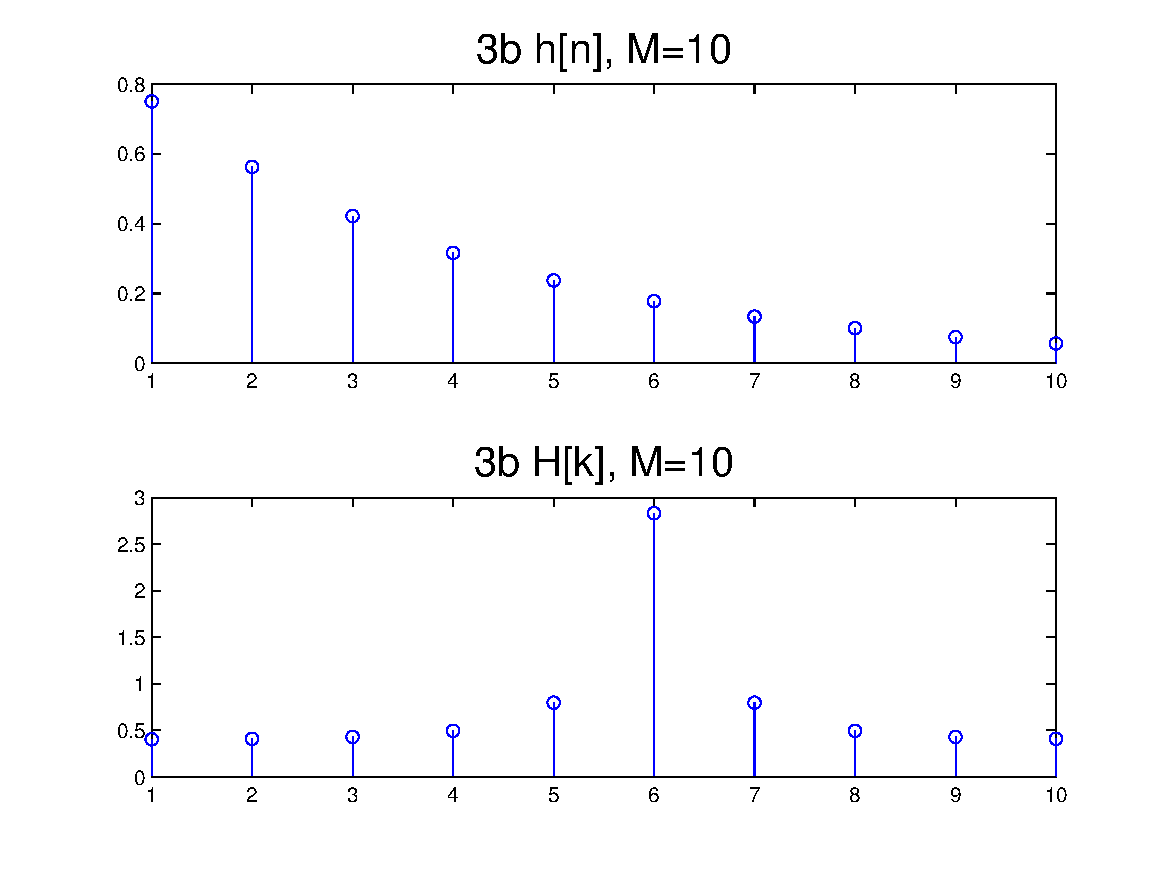
\includegraphics[width=.8\textwidth]{hw93b10-eps-converted-to.pdf} 
 
%  \includegraphics[width=.8\textwidth]{hw93b50}
  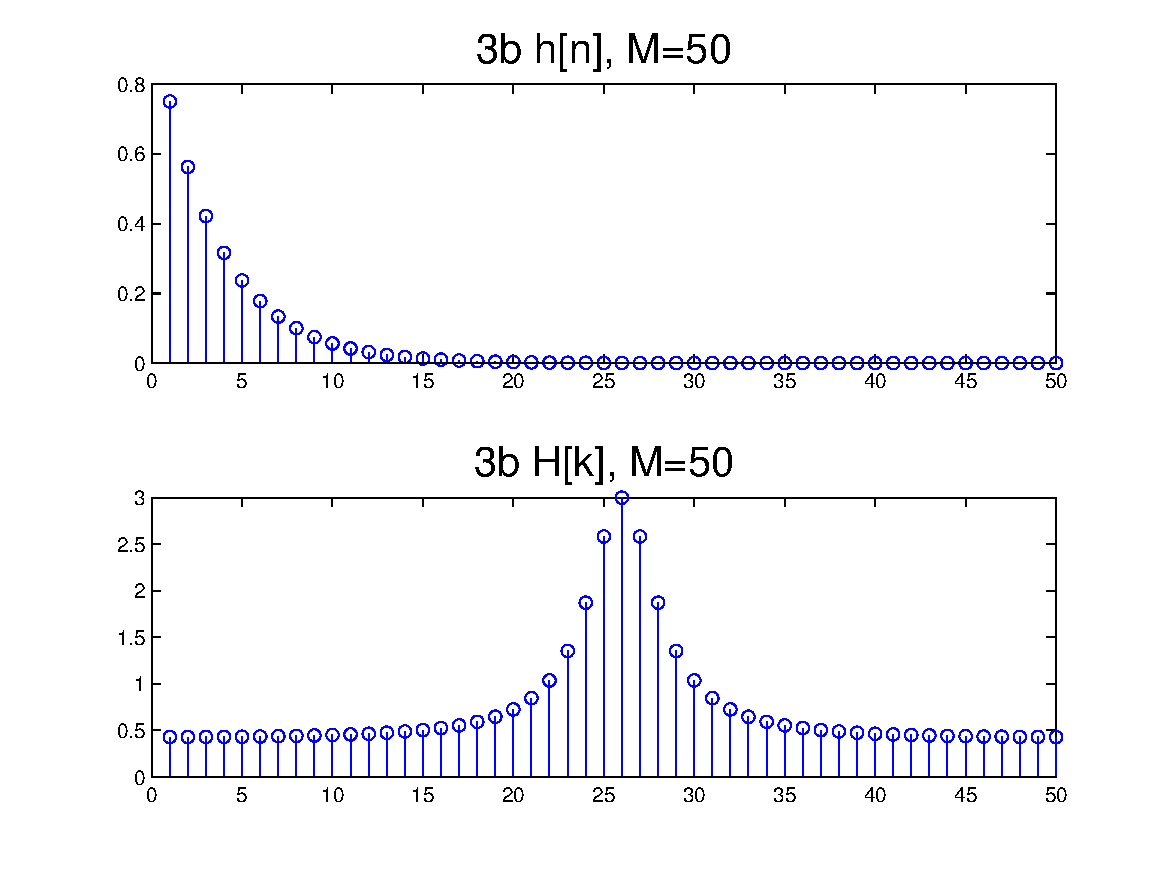
\includegraphics[width=.8\textwidth]{hw93b50-eps-converted-to.pdf}


\textbf{Solution.} We can see that the windowed impulse response with $M=50$ has a DFT that is more densely sampled. Graders: The plots are not required.


\vspace{3mm}
\item Using Matlab, window the impulse response with a Hamming window, Bartlett window, and Hanning window, all of length $M=50$. Their equations are found on p468 of the text. Qualitatively, how do the DFTs of these windowed impulse responses compare to one another? How do they compare to the rectangular window of length 50?

%  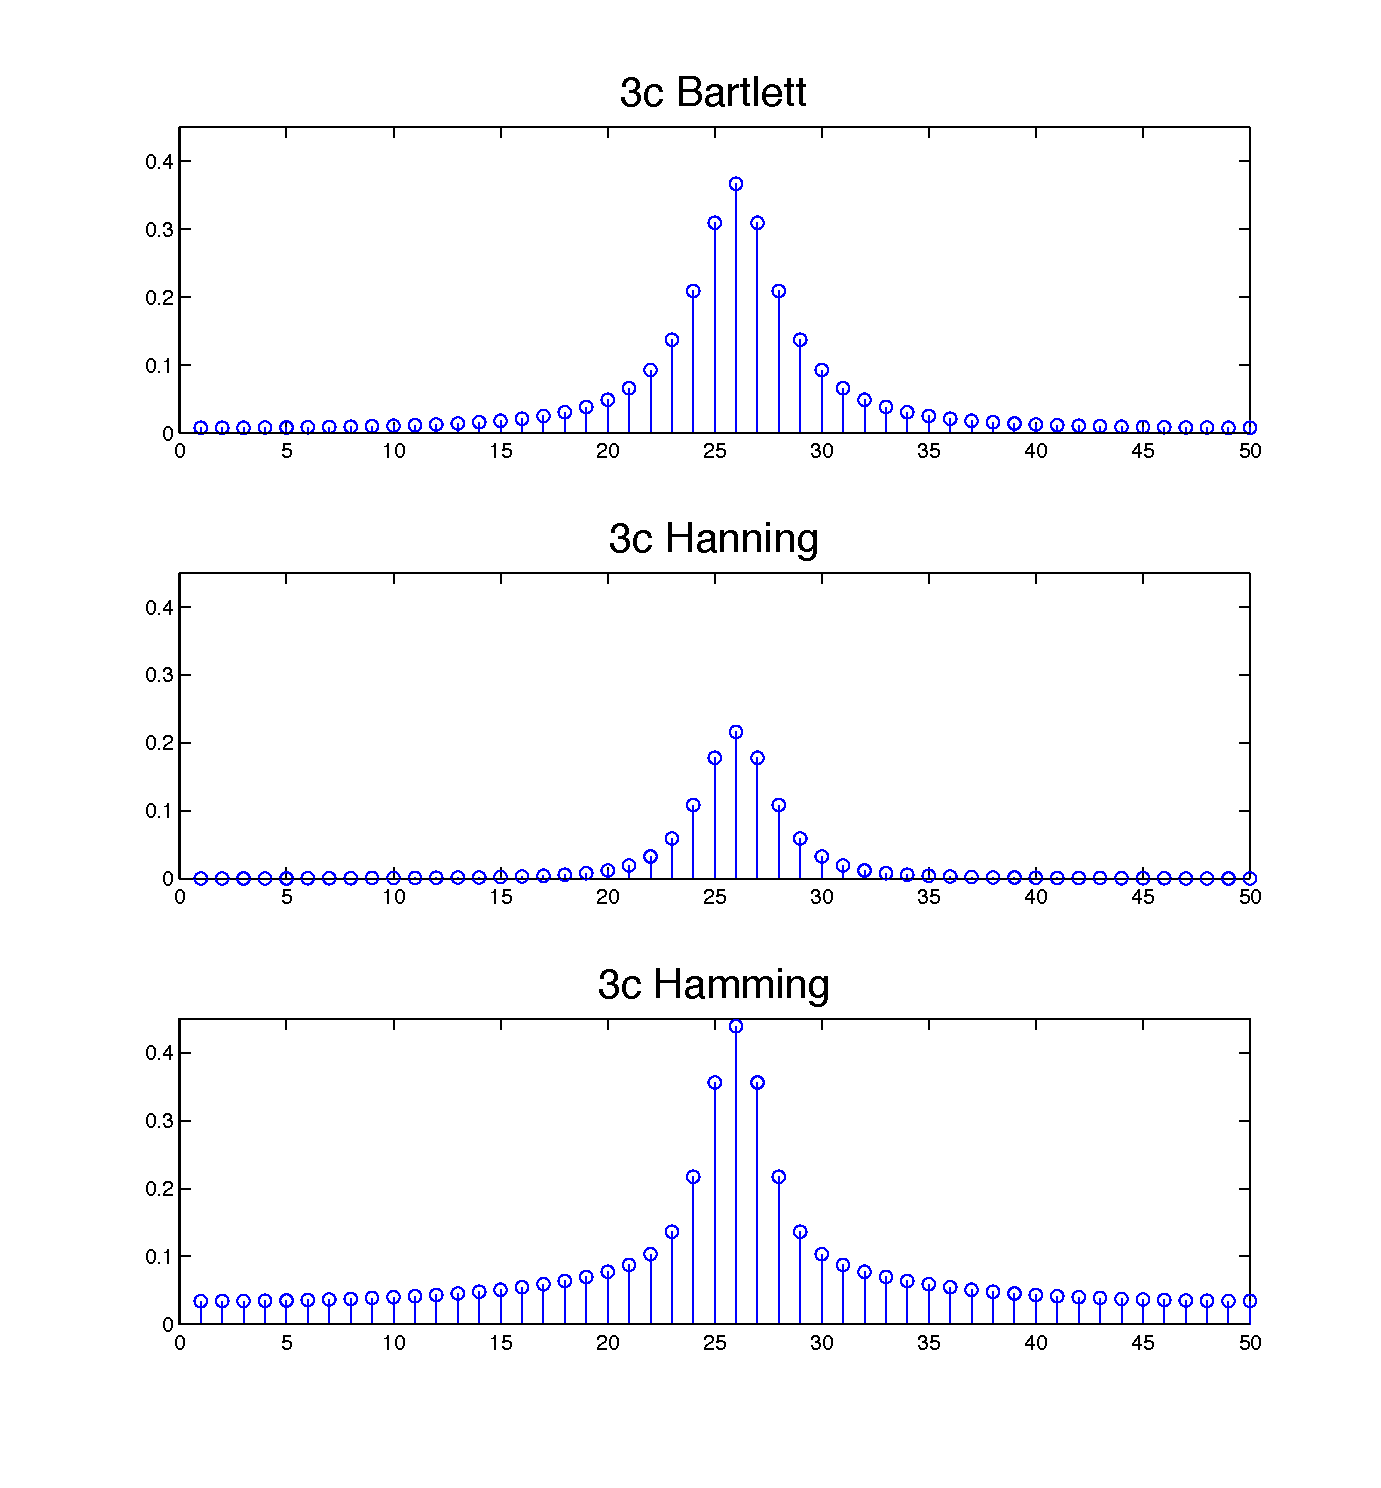
\includegraphics[width=.8\textwidth]{hw9windows}
  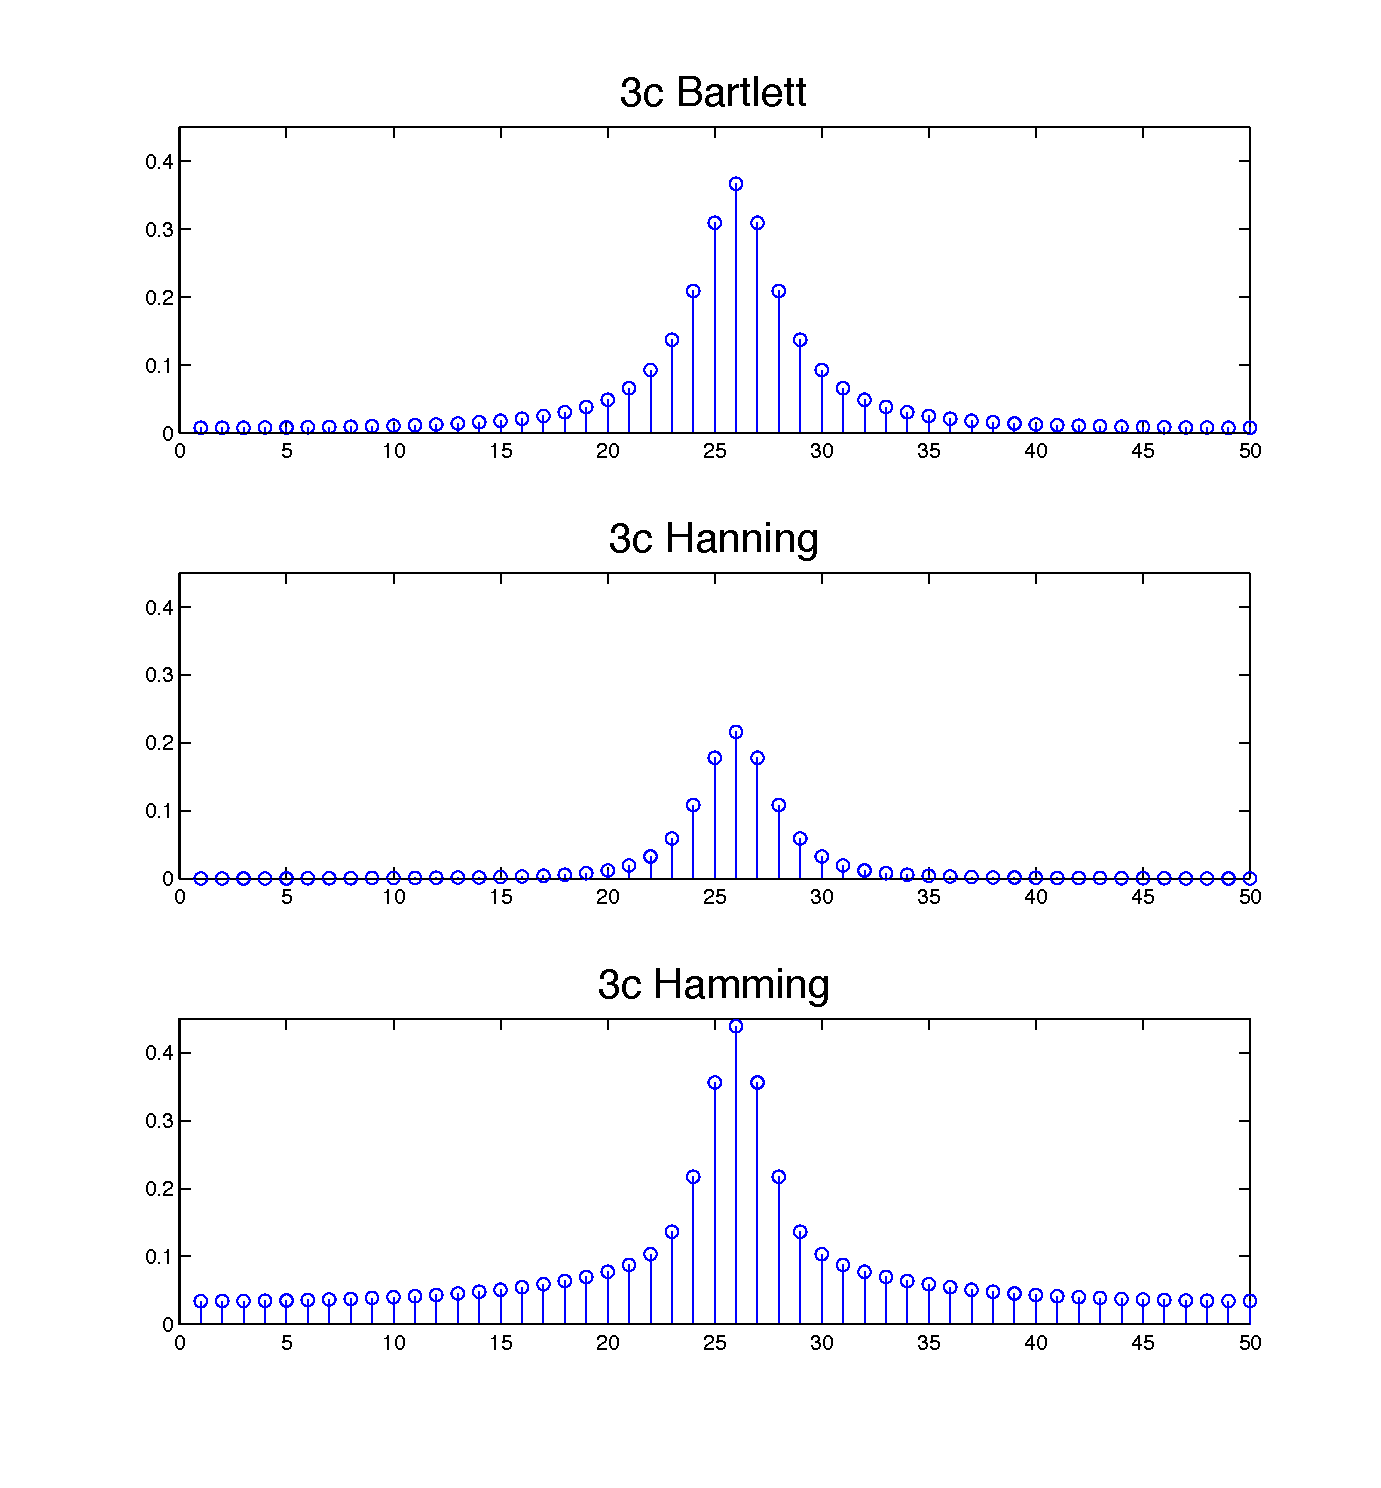
\includegraphics[width=.8\textwidth]{hw9windows.pdf}

\textbf{Solution.} The impulse response windowed by the Bartlett and Hamming windows are a little peakier in the center than the Hanning window. The tails of the Hanning windowed impulse response are very small. Graders: The plots or this specific comparison are not required; a general comparison is suitable for full credit.

\end{enumerate}


\newpage
\item Using the \texttt{fdatool} in matlab, design FIR lowpass filters of order 20 using the windowing method. Set the cutoff frequency to 4000 Hz. Try the hamming, kaiser (with beta=5), and rectangular window. Plot the magnitude and phase of the filter using freqz. What are the qualitative differences?

%  \includegraphics[width=.5\textwidth]{hw94hamming} 
   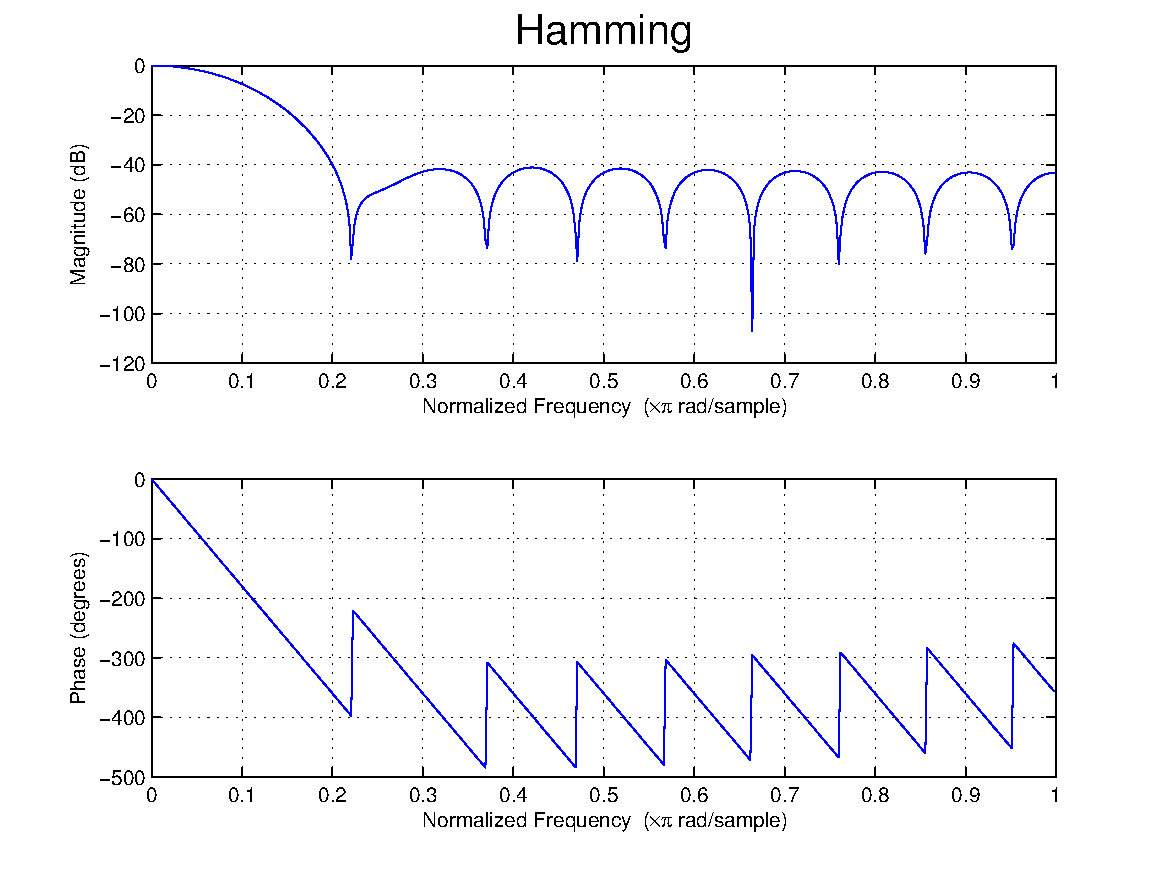
\includegraphics[width=.5\textwidth]{hw94hamming-eps-converted-to.pdf} 
 
%   \includegraphics[width=.5\textwidth]{hw94kaiser} 
   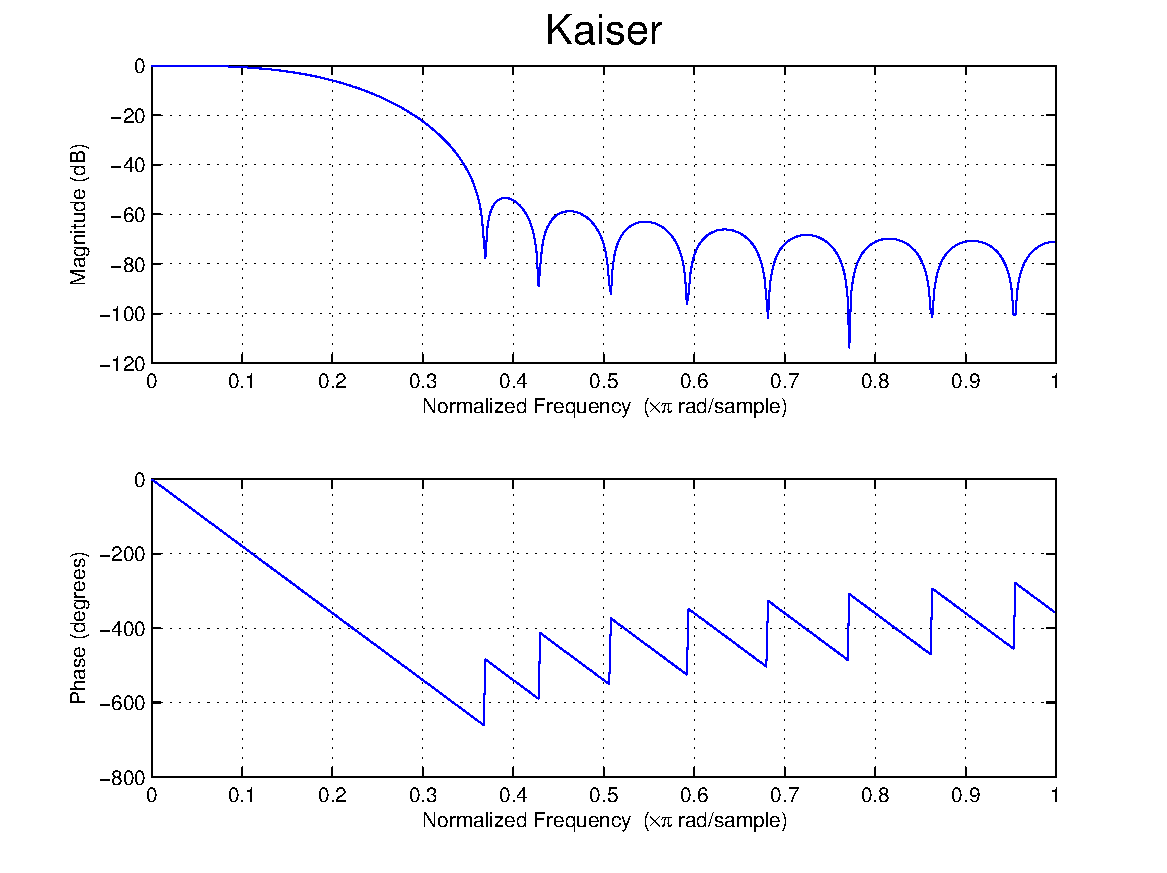
\includegraphics[width=.5\textwidth]{hw94kaiser-eps-converted-to.pdf} 
  
%   \includegraphics[width=.5\textwidth]{hw94rect}
   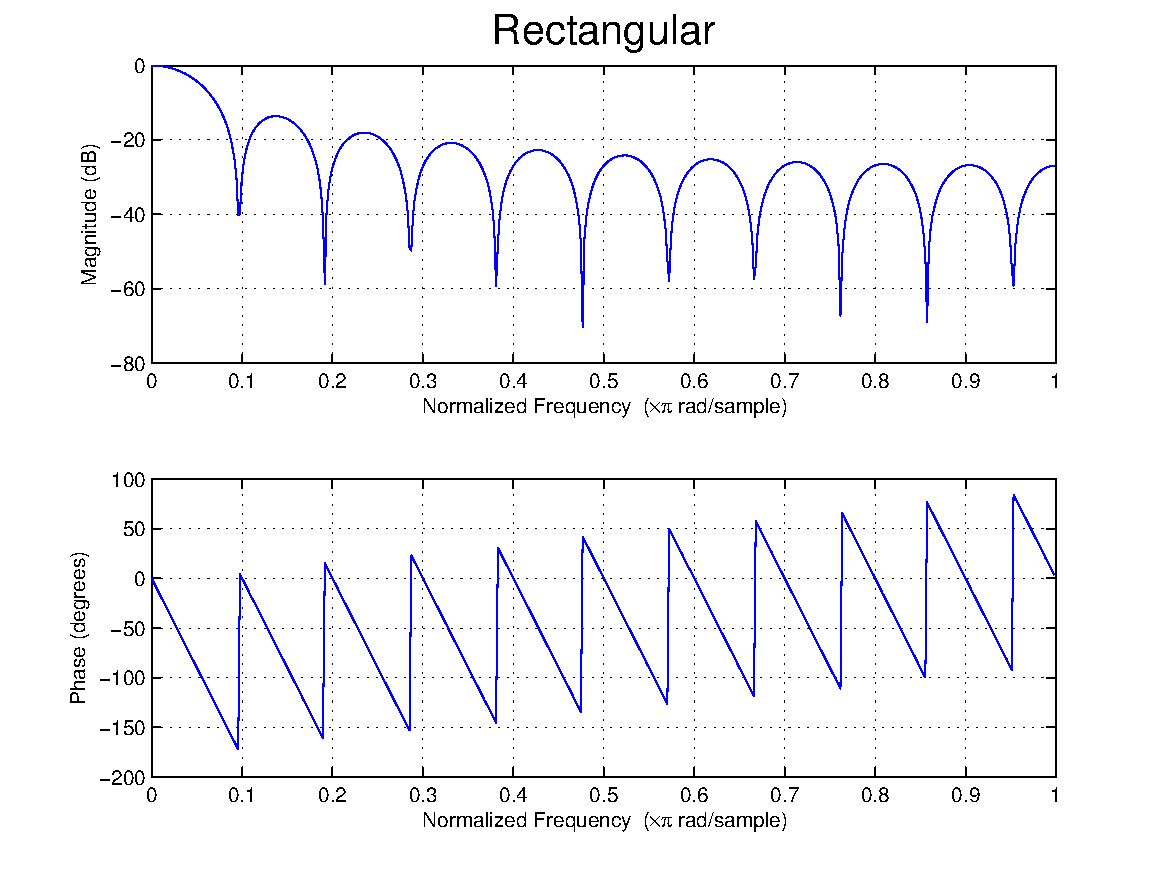
\includegraphics[width=.5\textwidth]{hw94rect-eps-converted-to.pdf}

\textbf{Solution.} The Kaiser window has a wider mainlobe and smaller sidelobes than either the Hamming or Rectangular, but its phase is not very uniform across the stopband. All of them have linear phase in the passband. The Hamming window has irregular magnitudes in the stopband. The Rectangular window has the smallest mainlobe and the highest sidelobes. Graders: The plots here are required, but again a general comparison is suitable for credit.


\newpage
\item A rare Jimi Hendrix recording was recently re-discovered at a recording studio. However, the (former) sound engineer did not protect against electromagnetic interference. Load the mat file at 

\noindent \url{http://web.eecs.umich.edu/~girasole/teaching/451/jimi.mat}

\noindent and listen to this short excerpt from the recording (the sampling rate is 8000 Hz). If your headphones have adequate low-frequency response, you will hear an annoying 120 Hz hum. 

\vspace{3mm}
\begin{enumerate}
\item Design an IIR notch filter by putting zeros at $z = e^{\pm j \omega_c}$ where $\omega_c = 2\pi 120/8000$ and poles at $r e^{\pm j \omega_c}$ where $r = 0.9$. What is the resulting difference equation (in the form of Equation~\ref{diff} above)? 

\vspace{3mm}
\item Using the \texttt{filter} command in matlab, apply this filter to the hendrix clip. Submit your code.
\end{enumerate}


\textbf{Solution.} We need zeros at $z=e^{\pm j\omega_c}$ where $\omega_c = 2 \pi 120/8000$. For an IIR notch filter we can put poles at $re^{\pm j \omega_c}$ for say, $r=0.9$. The resulting system function is 
\[ H(z)=\frac{(z-e^{j 0.03 \pi})(z-e^{-j0.03 \pi}) }{(z-0.9 e^{j 0.03 \pi})(z-0.9 e^{-j0.03 \pi}) }=\frac{z^2-2z \cos \omega_c +1 }{z^2 - 2rz \cos \omega_c + r^2} \]
where for this case $2 \cos \omega_c \approx 1.99$ and $2r \cos \omega_c \approx 1.79$. Thus the filter has the following difference equation:
\[ y[n] = 1.79 y[n-1] - 0.81 y[n-2] + x[n] - 1.99 x[n -1] + x[n-2]. \]
Here is the Matlab code.

\texttt{load 'jimi' \newline
a = [1 -1.79 0.81]; b = [1 -1.99 1]; \newline
y = filter(b,a,x);\newline
sound(y, 8000) \newline
figure; freqz(b, a, 100, 8000); \newline
figure; zplane(b,a); 
}

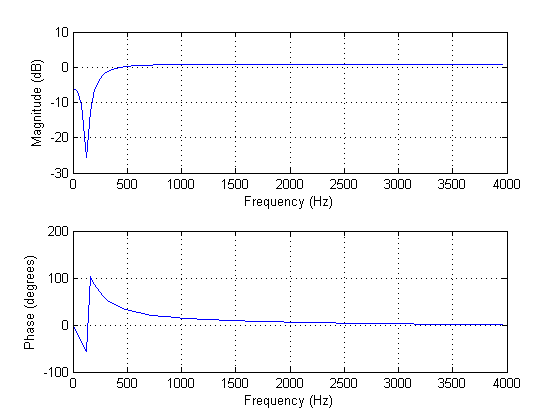
\includegraphics[width=0.8\textwidth]{notch_approx_freq_response.png} 

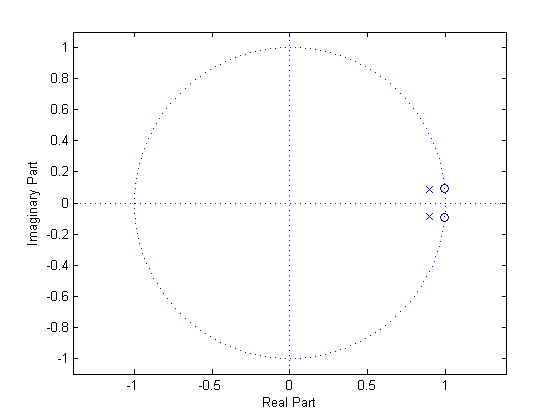
\includegraphics[width=0.8\textwidth]{notch_pole_zero.png}

Alternatively, you can get the $a_k$ and $b_k$ coefficients through use of Matlab's poly command:

\texttt{
omega\_c = 2*pi*120/8000;\newline
r = 0.9; \newline
zs = exp(j*[omega\_c -omega\_c]);\newline
ps = r*zs; \newline
b = poly(zs); \newline
a = poly(ps);}
This yields a slightly different frequency response:

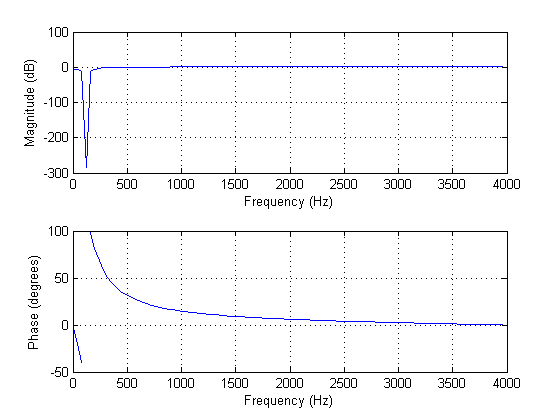
\includegraphics[width=0.8\textwidth]{notch_freq_response.png} 

The filter reduces the 120 Hz hum because of the "notch" in the magnitude response.


\end{enumerate}



\end{document}